%!TEX root = ../template.tex
%%%%%%%%%%%%%%%%%%%%%%%%%%%%%%%%%%%%%%%%%%%%%%%%%%%%%%%%%%%%%%%%%%%%
%% annex2.tex
%% NOVA thesis document file
%%
%% Chapter with example of appendix with a short dummy text
%%%%%%%%%%%%%%%%%%%%%%%%%%%%%%%%%%%%%%%%%%%%%%%%%%%%%%%%%%%%%%%%%%%%
\chapter{Annex 3 Bug on BTRFS affecting CoreUtils tool}
\label{ann:bug}

%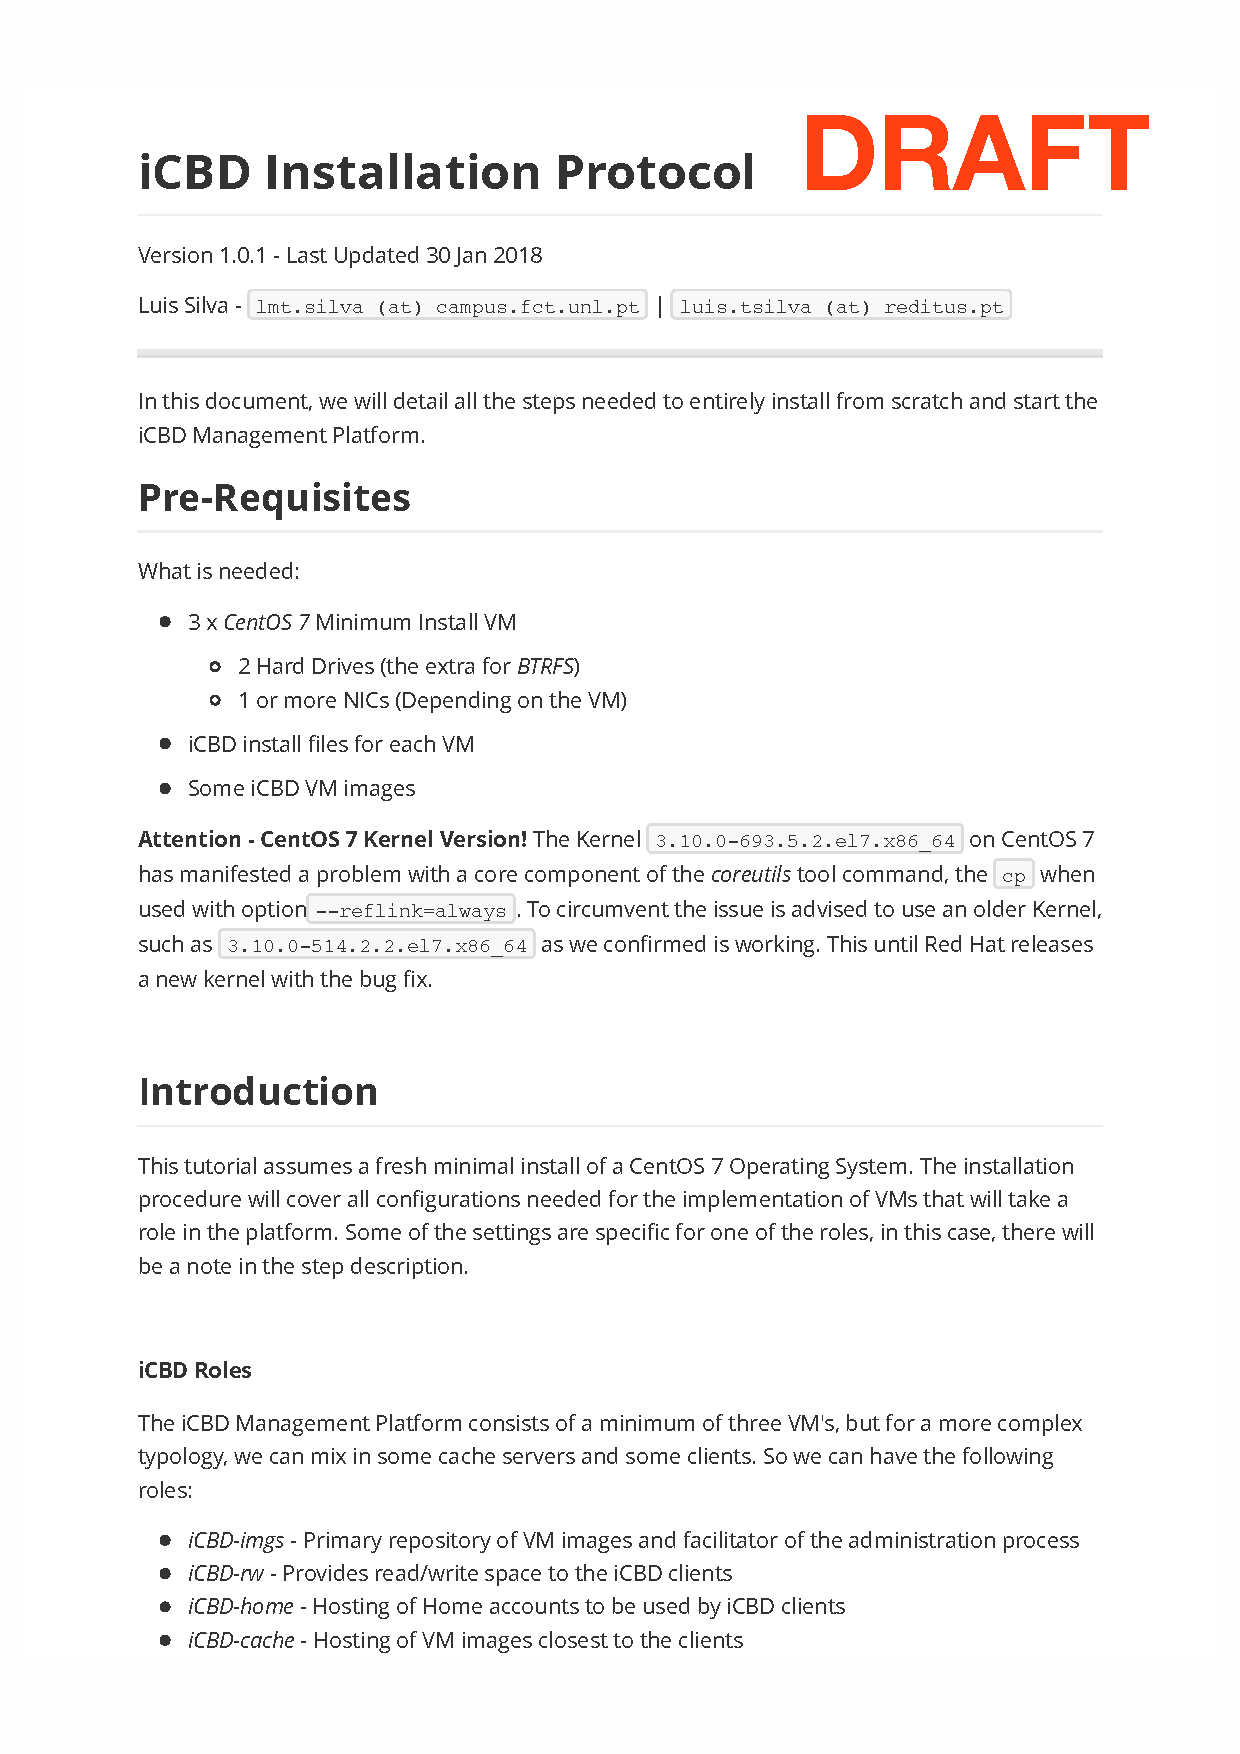
\includepdf[pages=-]{./Chapters/Annex/icbd_instalation_protocol_draft.pdf}

\section{Bug Report}
\label{sec:bug_report}

The bug was reported in both \textit{CentOS Bug Tracker} and \textit{Red Hat Bugzilla} on 4 of December of 2017.

\paragraph{Description of problem:}

In a CentOS 7 VM with kernel \texttt{3.10.0-693.5.2.el7.x86\_64} including a mounted disk formatted with BTRFS and btrfs-progs v4.9.1.
When executing a copy of files with the command \texttt{"cp --reflink=always"} the command fails with the indication \textit{"failed to clone 'someFile': Operation not supported"}

\paragraph{Issue:}

The above-mentioned copy fails, but in the files are created with zero bytes in the destination folder.
While trying to find the cause, it seems to be some bug in the ioctl operation. A strace log of the copy operation can be found in the uploaded files.

This problem only manifests itself in the kernel \texttt{3.10.0-693.5.2.el7.x86\_64}. If the same operation is executed in the system with the kernel \texttt{3.10.0-514.2.2.el7.x86\_64} all goes well.
More evidence that this is probably a bug introduced in this version of the kernel can be found in the git repository in the first commit of the new kernel~\footnote{https://git.centos.org/commit/rpms!kernel.git/d6bfd60741b14479a15b43acaa1ea5a8d73df543}.
In the file "SPECS/kernel.spec" line 15011~\footnote{https://git.centos.org/blob/rpms!kernel.git/d6bfd60741b14479a15b43acaa1ea5a8d73df543/SPECS!kernel.spec\#L15011} that some changes were made in the ioctl - \textit{"[fs] btrfs: fix uninit variable in clone ioctl (Bill O'Donnell) [1298680]"}

As a workaround, an older version of the kernel can be used, but this is not optimal, as future releases may have the same problem.

\paragraph{How reproducible:}

It is always reproducible. Happens every time.

\paragraph{Steps to Reproduce:}

\begin{enumerate}
	\item In a BTRFS mount execute:
	\item \texttt{dd if=/dev/urandom of=testb bs=1024k seek=1024 count=128}
	\item \texttt{cp --reflink=always testb testb\_copy}
\end{enumerate}

\paragraph{Actual results:}
The copy operation returns with "failed to clone 'testb': Operation not supported" and creates a zero bytes file in the destination of the copy.

\paragraph{Expected results:}

A clone of the file, looking precisely the same as the original with the same size.

\begin{listing}[h!]
\begin{minted}[frame=lines, framesep=2mm, fontsize=\footnotesize, linenos]{python}
execve("/usr/bin/cp", ["cp", "--reflink=always", "testb", "test_reflink"], [/* 33 vars */]) = 0
(...)
access("/etc/selinux/config", F_OK)     = 0
open("/usr/lib/locale/locale-archive", O_RDONLY|O_CLOEXEC) = 3
fstat(3, {st_mode=S_IFREG|0644, st_size=106070960, ...}) = 0
mmap(NULL, 106070960, PROT_READ, MAP_PRIVATE, 3, 0) = 0x7f43ee219000
close(3)                                = 0
open("/usr/share/locale/locale.alias", O_RDONLY|O_CLOEXEC) = 3
fstat(3, {st_mode=S_IFREG|0644, st_size=2502, ...}) = 0
mmap(NULL, 4096, PROT_READ|PROT_WRITE, MAP_PRIVATE|MAP_ANONYMOUS, -1, 0) = 0x7f43f59db000
read(3, "# Locale name alias data base.\n#"..., 4096) = 2502
read(3, "", 4096)                       = 0
close(3)                                = 0
munmap(0x7f43f59db000, 4096)            = 0
open("/usr/lib/locale/UTF-8/LC_CTYPE", O_RDONLY|O_CLOEXEC) = -1 ENOENT (No such file or directory)
geteuid()                               = 0
stat("test_reflink", {st_mode=S_IFREG|0644, st_size=0, ...}) = 0
stat("testb", {st_mode=S_IFREG|0644, st_size=1207959552, ...}) = 0
stat("test_reflink", {st_mode=S_IFREG|0644, st_size=0, ...}) = 0
open("testb", O_RDONLY)                 = 3
fstat(3, {st_mode=S_IFREG|0644, st_size=1207959552, ...}) = 0
open("test_reflink", O_WRONLY|O_TRUNC)  = 4
fstat(4, {st_mode=S_IFREG|0644, st_size=0, ...}) = 0
ioctl(4, BTRFS_IOC_CLONE or FICLONE, 3) = -1 EOPNOTSUPP (Operation not supported)
open("/usr/lib64/charset.alias", O_RDONLY|O_NOFOLLOW) = -1 ENOENT (No such file or directory)
write(2, "cp: ", 4)                     = 4
write(2, "failed to clone 'test_reflink' f"..., 43) = 43
write(2, ": Operation not supported", 25) = 25
write(2, "\n", 1)                       = 1
close(4)                                = 0
close(3)                                = 0
lseek(0, 0, SEEK_CUR)                   = -1 ESPIPE (Illegal seek)
close(0)                                = 0
close(1)                                = 0
close(2)                                = 0
exit_group(1)                           = ?
+++ exited with 1 +++
\end{minted}
\caption{Strace of the \texttt{cp --reflink=always} command}
\label{listing:icbd_nameserver}
\end{listing}


\section{Resolution}
\label{sec:resolution}
On 5 of April of 2018, the problem was acknowledged by Red Hat, and a patch was provided. However, also informed that the fix would be included in later RHEL7 releases, due to Red Hat deciding to deprecate BTRFS as of RHEL7.5.

\begin{listing}[h!]
\begin{minted}[frame=lines, framesep=2mm, fontsize=\footnotesize, linenos]{python}
--- a/fs/btrfs/super.c	
+++ a/fs/btrfs/super.c	
@@ -2191,7 +2191,7 @@ static struct file_system_type btrfs_fs_type = {
 	.name		= "btrfs",
 	.mount		= btrfs_mount,
 	.kill_sb	= btrfs_kill_super,
-	.fs_flags	= FS_REQUIRES_DEV | FS_BINARY_MOUNTDATA,
+	.fs_flags	= FS_REQUIRES_DEV | FS_BINARY_MOUNTDATA | FS_HAS_FO_EXTEND,
 };
 MODULE_ALIAS_FS("btrfs");
\end{minted}
\caption{BTRFS patch on a/fs/btrfs/super.c}
\label{listing:icbd_nameserver}
\end{listing}


